%%% BEN 5' %%%

\section{Bestimmung der Relaxationszeit nach Dehmelt}
\subsection{Grundlagen: Relaxationsprozesse}

\begin{frame}
\frametitle{Grundlagen: Relaxationsprozesse beim optischen Pumpen}
\begin{itemize}[<+->]
    \item Pumpzeit $T_\text{P}$
    \begin{equation*}
        \left(\frac{\difd n}{\difd t}\right)_{\text{Pump}}=\frac{N-n}{T_\text{P}}
    \end{equation*}
    $N$: Anzahl der Atome in Ensemble, $n$: Differenz der Besetzungszahlen
    \item Relaxation durch
    \begin{itemize}[<+->]
        \item Wechselwirkung mit Wand der Messzelle
        \item Stöße mit dem Puffergas
        \item Spinaustausch zwischen Rubidiumatomen
    \end{itemize}
    \item Relaxationszeit $T_\text{R}$
    \begin{equation*}
        \left(\frac{\difd n}{\difd t}\right)_{\text{Relax}}=-\frac{n}{T_\text{R}}
    \end{equation*}
\end{itemize}
\end{frame}

\begin{frame}
\frametitle{Grundlagen: Relaxationsprozesse beim optischen Pumpen}
\begin{itemize}[<+->]
    \item Orientierungsprozess
    \begin{equation*}
        \left(\frac{\difd n}{\difd t}\right)_{\text{Orient}}
        =\left(\frac{\difd n}{\difd t}\right)_{\text{Pump}} + \left(\frac{\difd n}{\difd t}\right)_{\text{Relax}}
        =\frac{N}{T_\text{P}}-n \left( \frac{1}{T_\text{P}} + \frac{1}{T_\text{R}}\right)
    \end{equation*}
    \item Orientierungszeit $\tau$
    \begin{equation*}
        \begin{split}
            & \left(\frac{\difd n}{\difd t}\right)_{\text{Orient}} = \frac{N}{T_\text{P}}- \frac{n}{\tau} \\
            & \frac{1}{\tau} := \frac{1}{T_\text{P}} + \frac{1}{T_\text{R}}
        \end{split}
    \end{equation*}
    \item Pumpzeit $T_\text{P}$ ist umgekehrt proportional zur Intensität $I$
    \begin{equation*}
        \frac{1}{T_\text{P}} = \alpha I
    \end{equation*}
\end{itemize}
\end{frame}

\subsection{Aufbau}
\begin{frame}
\frametitle{Aufbau Dehmelt}

\setbeamerfont{myfont}{size*=80}
\usebeamerfont{myfont}
\begin{figure}
    \centering
    \def\svgwidth{\textwidth}
    \input{../img/aufbaudehmelt.pdf_tex}
    \caption{Aufbau..}
\end{figure}
\usebeamerfont{standard}

\begin{itemize}
    \item \textbf{ND-Filter:} Abschwächung der Laserintensität um 60\% bis 98\%
    \item \textbf{Spule 3:} Rechteckiges Wechselfeld mit 50\,Hz
    \item \textbf{Spule 4:} Kompensation von vertikalem Erdmagnetfeld
\end{itemize}
\end{frame}

%TODO Evtl Pumpschema für mf=2 -> mf=-2

\subsection{Auswertung}
\begin{frame}
\frametitle{Auswertung: Dehmelt}
\begin{figure}
    \begin{center}
        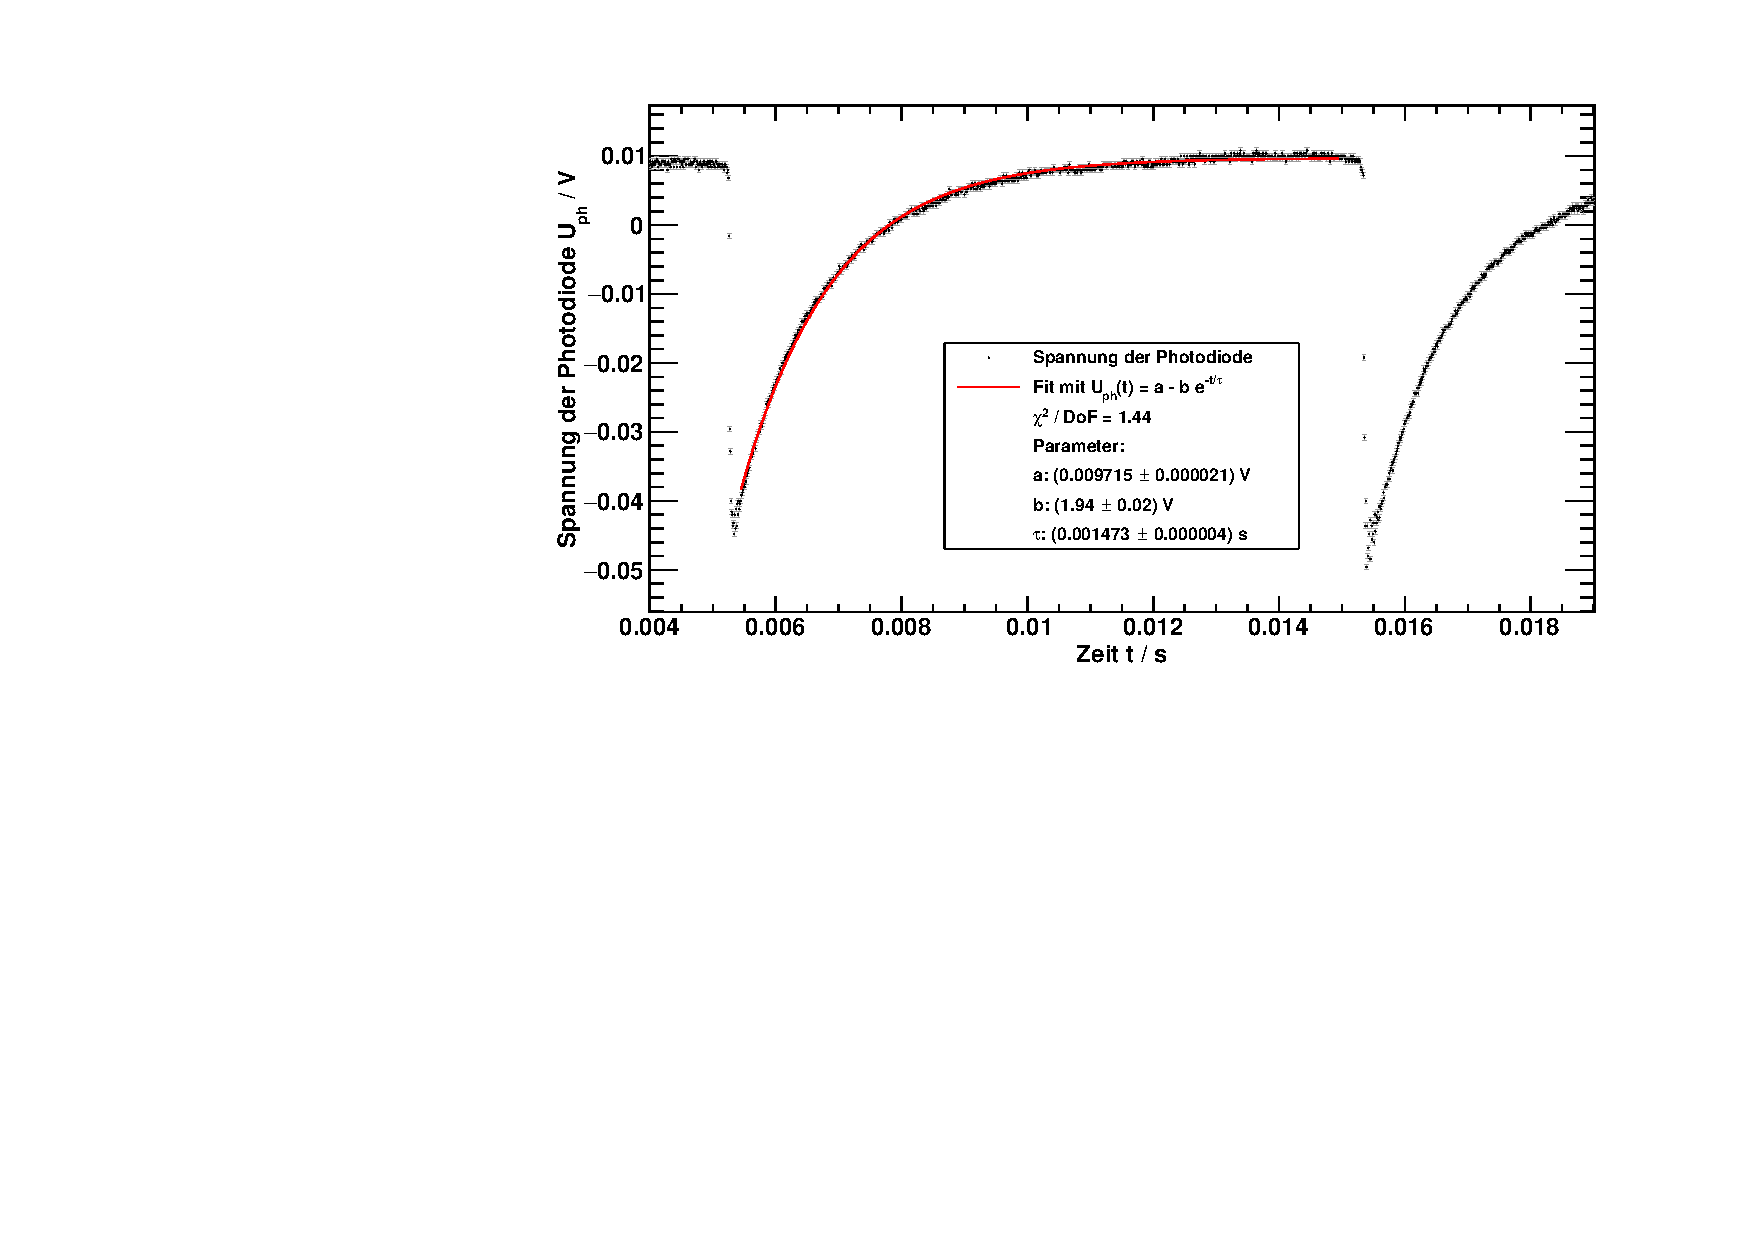
\includegraphics[width=\textwidth]{../img/65-5mA-10.pdf}
        \caption{Spannung der Photodiode (entspricht der Transmission durch die Rubidiumzelle)
        nach Umkehr des Magnetfelds.
        Die Orientierungszeit $\tau$ des Fits wird durch Polarisations- und Relaxationsprozesse bestimmt.}
    \end{center}
\end{figure}
\end{frame}

\begin{frame}
\frametitle{Auswertung: Dehmelt}
\begin{itemize}[<+->]
    \item Fit mit
    \begin{equation*}
        U_{\text{ph}}(t)=a - b \cdot e^{-\frac{t}{\tau}}
    \end{equation*}
    für verschiedene Intensitäten
    \item Fit der Orientierungszeiten $\tau(I)$ 
    \begin{equation*}
        \frac{1}{\tau(I)}=\alpha I + \frac{1}{T_{\text{R}_\text{D}}}
    \end{equation*}
\end{itemize}
\end{frame}

\begin{frame}
\frametitle{Auswertung: Dehmelt}
\begin{figure}
    \begin{center}
        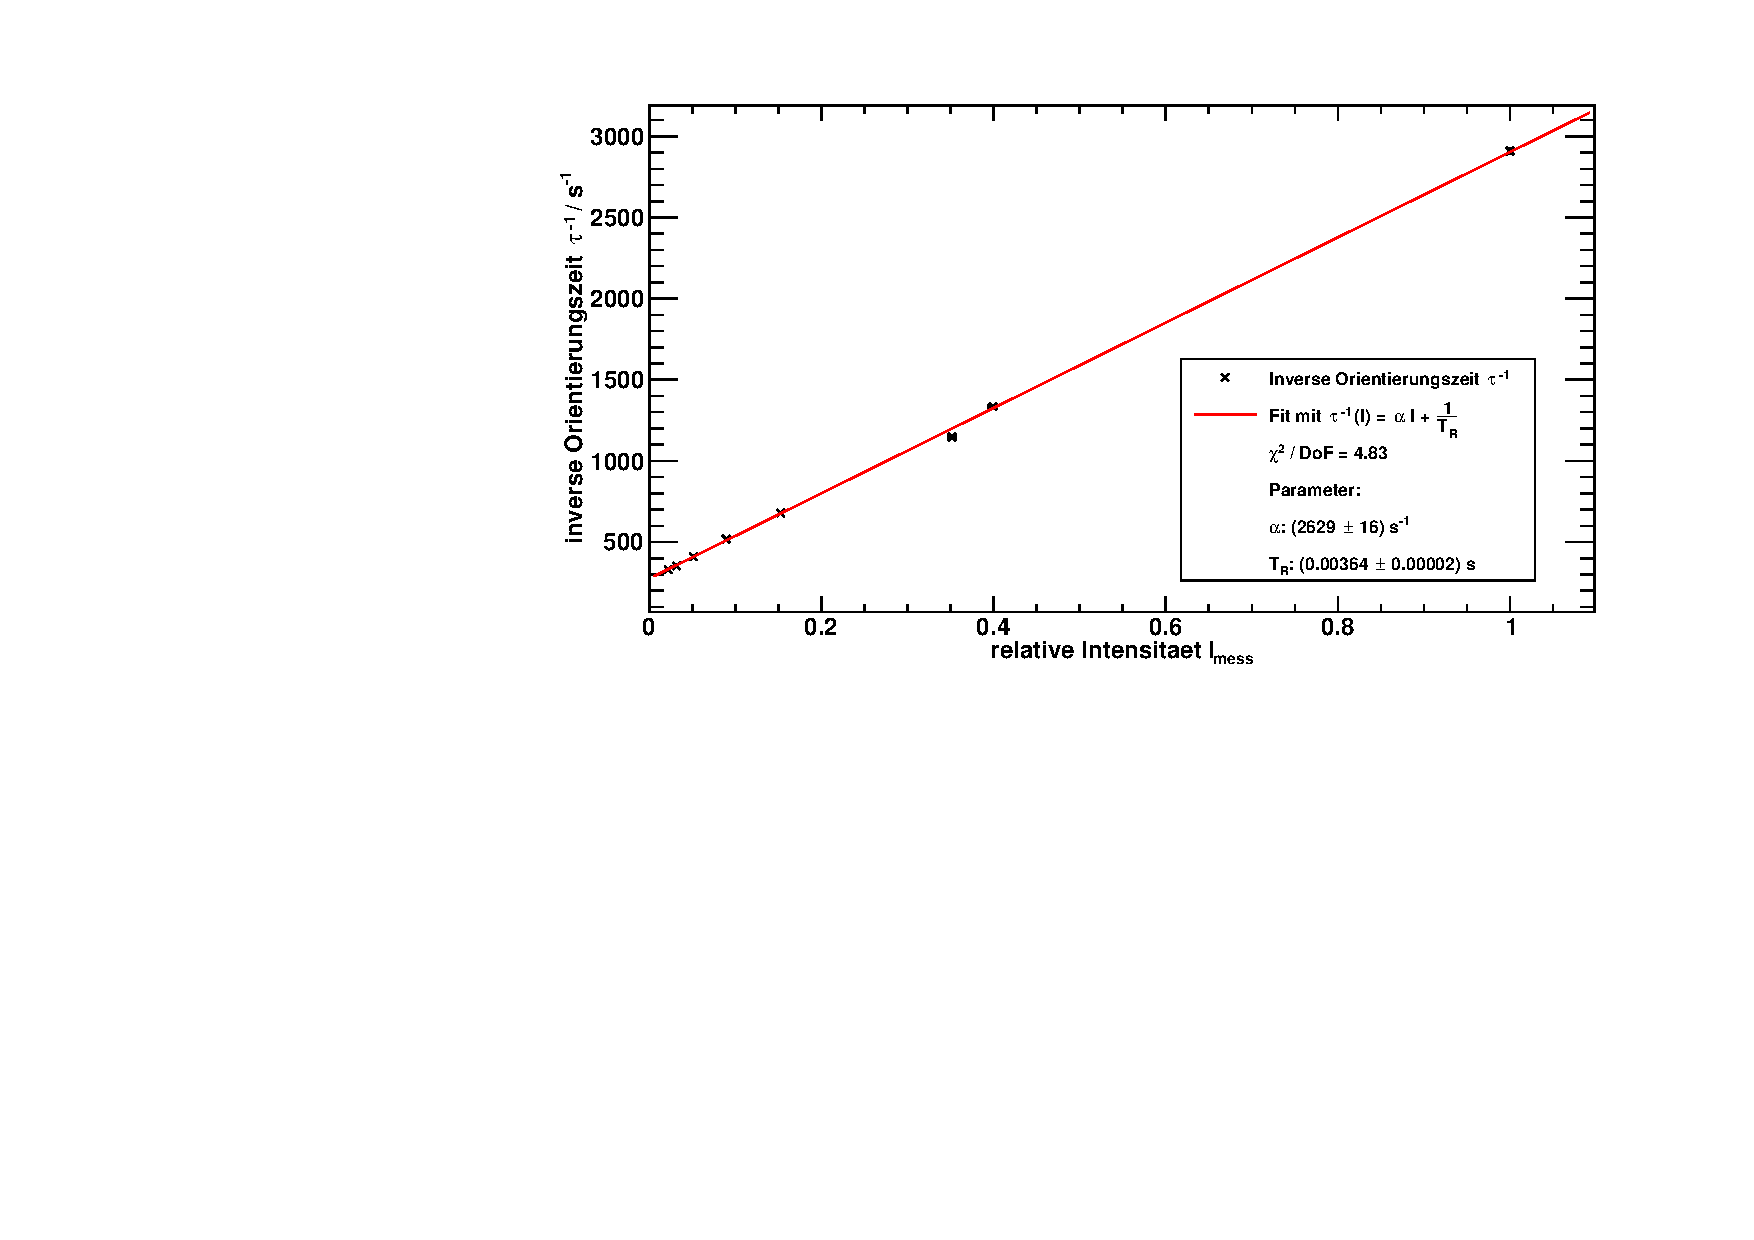
\includegraphics[width=\textwidth]{../img/taufit.pdf}
        \caption{Extraktion der Relaxationszeit $T_{\text{R}_\text{D}}$ aus den Messdaten für die Orientierungszeit~$\tau$.}
    \end{center}
\end{figure}
\end{frame}

\begin{frame}
\frametitle{Ergebnis: Dehmelt}
\begin{itemize}[<+->]
    \item Relaxationszeit
    \begin{equation*}
        T_{\text{R}_\text{D}} = 3.64 \pm 0.02\,\text{ms}
    \end{equation*}
    \item Literaturwert
    \begin{equation*}
        T_{\text{R}_\text{D}}^\text{Lit.} = 6.5\,\text{ms}
    \end{equation*}
    \item Mögliche Fehlerquelle: Andere Mechanismen
\end{itemize}
\end{frame}